\documentclass[a4paper,14pt]{book}

\usepackage[utf8]{inputenc}
\usepackage[T1]{fontenc}

\usepackage{lmodern}
\usepackage{epigraph}
\usepackage{graphicx}

\usepackage[a4paper, left=2cm, top=2cm, right=2cm, bottom=2cm]{geometry}

\renewcommand{\chaptername}{Capítulo}

\title{\Huge Contos do Sistema Solar}
\author{Giseldo Neo}

\begin{document}

\newgeometry{left=0cm, top=0cm, right=0cm, bottom=0cm}
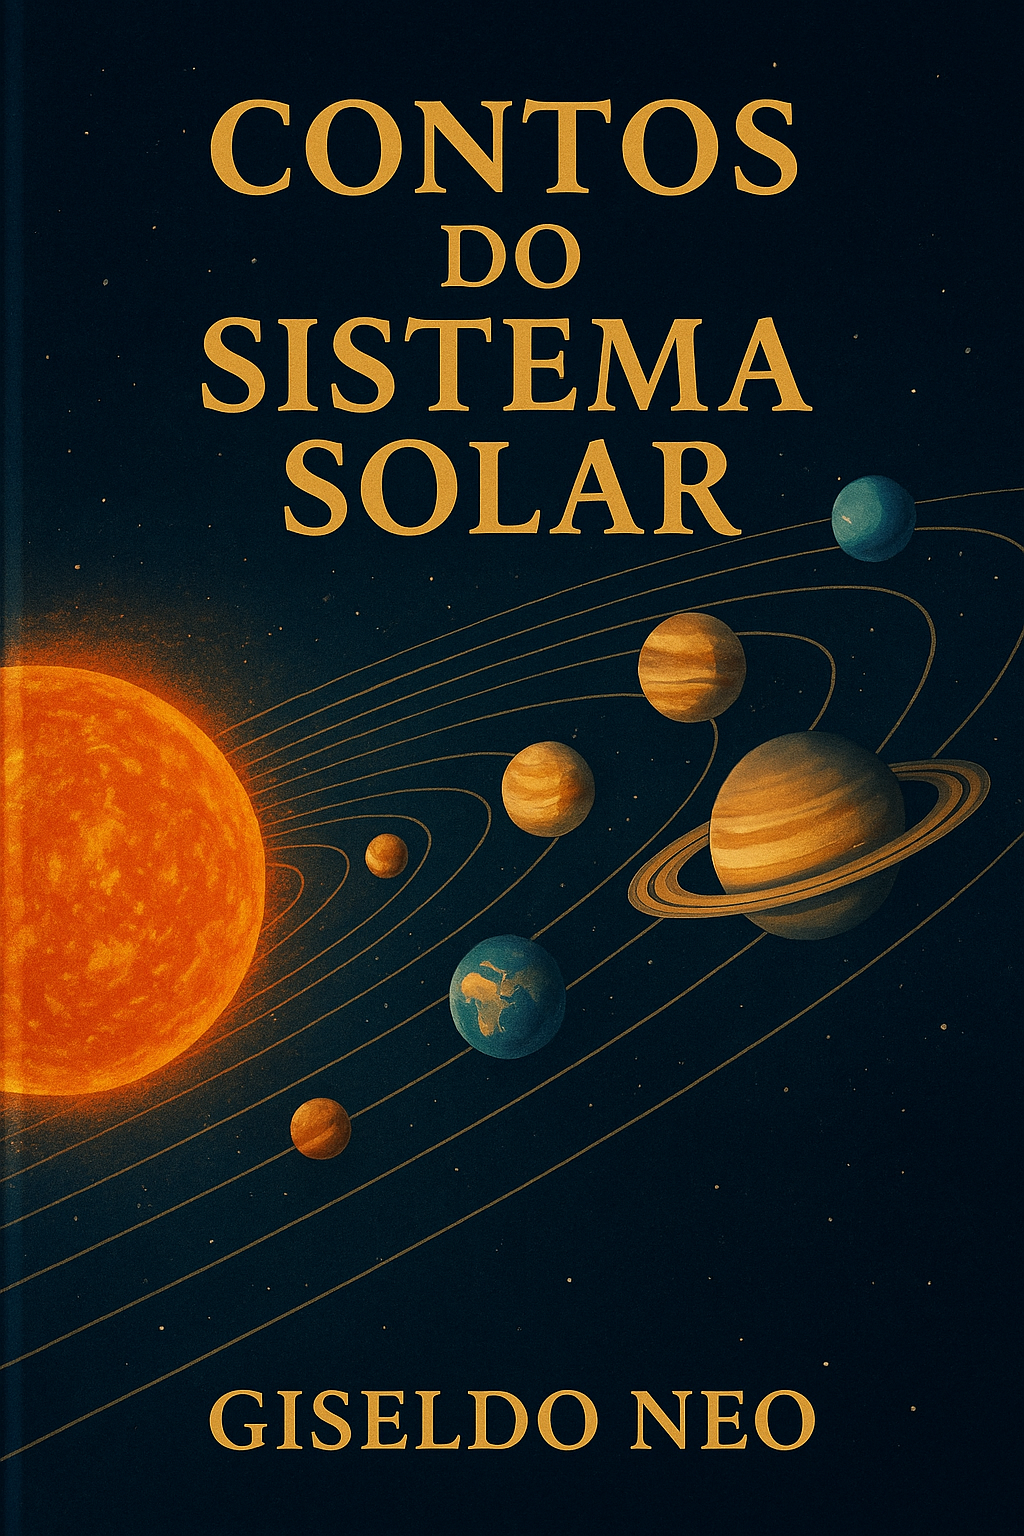
\includegraphics[width=\textwidth,height=\textheight,keepaspectratio]{img/capa.png}
\restoregeometry

% \maketitle

\LARGE

\chapter*{Prefácio}

Lembro de ter sido feliz lendo livros de ficção. Conhecer aquelas histórias e mundos diferentes me instigava. Recordo, com nostalgia, o encantamento dos livros-jogos de Ian Livingstone e Steve Jackson. Eles eram vendidos em sebos, suas capas eram incríveis; a possibilidade de escrever a sua própria história com estes livros marcou a minha infância.

Na escola, fui apresentado à série Vaga-lume e aos clássicos de nossa literatura. Alguns me interessavam mais que outros, e acho que é assim que deve ser, em algum momento um daqueles autores toca no interior do leitor de forma única. Aconteceu comigo com “Noites na Taverna”, de Álvares de Azevedo, foi um êxtase. Aquelas histórias de boêmios românticos orgulhosos (ou tristes) cometendo crimes contra mulheres, assassinando pessoas, brindando  suas vidas desgarradas, endeusando mulheres, falando da morte como algo corriqueiro foi uma experiência única.

Além disso, outros livros, como Casa de Pensão e Cortiço, também me interessavam, aquela linguagem naturalista falando do dia-a-dia de forma quase poética, como um artista pintando um lindo quadro de uma paisagem comum. Com estes livros, o mundo, assim como eu o percebia, ganhou um significado maior. As nuances da vida cotidiana ganharam novos contornos.

Todo esse encantamento com a leitura teve grande influência da escola e dos professores, que montaram um currículo com tais livros; dos autores que o escreveram; e dos meus pais que pagaram com seu suor enquanto eu estudava. Não precisei trabalhar na infância, tive o tempo do ócio, da diversão, das amizades, do descanso, das brincadeiras, da TV, do estudo, dos videogames e da leitura. 

Em meados de 1995, a internet chegou ao Brasil e com ela as possibilidades de leitura e acesso a livros aumentaram. Entrar na grande rede, falar com outras pessoas e ler livros de ficção, tais como Arthur Clark e Philip K. Dick, foi uma re-descoberta.

A escrita de Dick era rápida, cotidiana, acontecia no futuro, era como unir dois mundos, levar o leitor a outras realidades e contar as histórias de sua realidade. Pois escrever ficção é mais refletir sobre o presente do que discursar sobre o futuro. Philip K. Dick não viveu para ver o reconhecimento de suas obras. Viveu as dificuldades que a maioria de nós vive, isso está nas entrelinhas de seu texto, geralmente personagens comuns, com problemas comuns. Hoje, um aclamado autor, que influenciou e influencia nossa visão de mundo.

Um escritor se comunica com o leitor mesmo depois de sua morte.
É como viajar no tempo. Se comunicar com outros mesmo não estando presente. Quero fazer isto com estes contos. Eles foram escritos com carinho. Espero que o leitor interessado o aprecie, como aconteceu comigo no passado. Se ao menos um jovem se divertir com essa obra e lembrar destas histórias, já terá valido a pena.

\begin{flushright}
Giseldo Neo
\end{flushright}

\chapter*{Agradecimentos}
Agradeço aos meus antepassados, não quero decepcioná-los. A família que me gerou, nutriu e amou. A nova família, que construímos, eu e minha esposa. Tenho filhas lindas. Tive um bom tempo no mundo.

\chapter{A Escuridão de Nova Europa}

\epigraph{A coragem não é a ausência de medo, mas o triunfo sobre ele}{Aristóteles}

\begin{figure}[h!]
    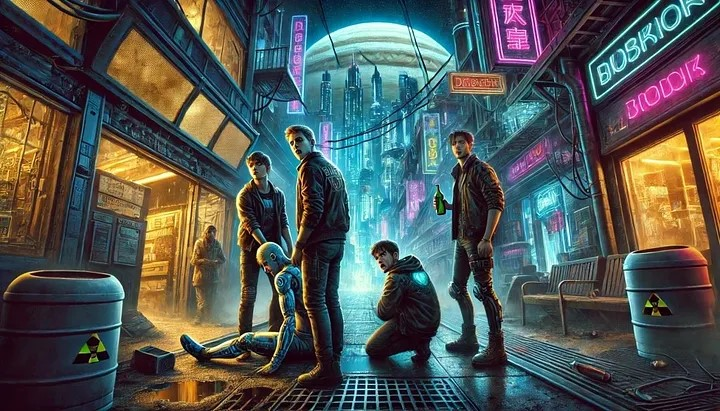
\includegraphics[width=1\linewidth]{img/a_escurida_de_nova_europa.jpg}
\end{figure}

O condapt começou a ser iluminado lentamente. O ciclo da manhã estava iniciando. As notícias mais importantes do dia foram projetadas na mesa no outro canto do pequeno espaço. Não havia tempo para se barbear, pensou. Olhou-se no espelho e percebeu que a sua barba era rala e mal crescia. Iria esperar mais um ano antes do procedimento definitivo a laser, que só poderia ser feito aos 20 anos.

— O escudo de radiação ao redor de Nova Europa reteve hoje 95\% — afirmava um humano-robô do lado de fora da redoma.

— Em uma década, a situação estará insustentável para humanos não modificados.

Robert saiu para o trabalho diário, ao fechar a porta, todas as luzes se apagaram e a projeção holográfica do jornal encerrou. Teve todo o tempo do mundo para uma boa refeição, nessa manhã artificial.

As manhãs de Nova Europa não eram como na terra ou em luna. Nova Europa não girava como um planeta ao redor do eixo, e mantinha parte escura e parte iluminada. O plano de fazer o planeta girar com a energia nuclear falhou e explodiu, matando alguns humanos-robôs. Mas ele não se importava, como chegara à lua de Júpiter quando ainda era pequeno, não sentia falta do que nunca teve.

Ele trabalhava para o Governo Central, o que lhe permitia viver com certa dignidade. Um condapt, um espaço de 5 por 5 metros quadrados, para si era um luxo em um ambiente com espaço confinado e com reserva de oxigênio. Seu trabalho consistia em entender e escrever as equações da teoria-de-tudo, que substitui a teoria da relatividade, sempre se considerou com sorte.

No final do expediente, depois de suas refeições, foi ao encontro da festa do fim do mundo, a festa do mês de julho, que acontecia próximo ao depósito de reciclagem. Sempre havia boas festas e locais para entretenimento de todos os gostos, inclusive os duvidosos, em toda a redoma.

Ao chegar no portão de identificação, encontrou 4 amigos, um era de estatura baixa, outro tinha um boné na cabeça, um com uma perna mecânica e outro sorridente.

— Trouxe a cachaça conforme combinado. Disse o Baixinho, com uma garrafa contrabandeada do sul-global da antiga terra. — Tome um gole, que chegamos cedo e já estamos quentes.

Robert sugou o líquido de um canudo metálico, de um recipiente que parecia uma bolsa de sangue, era amargo, desceu queimando. Em poucos minutos, ficou relaxado e logo depois eufórico.

— Difícil a vida sem uma boa cachaça. Vamos entrar, a noite é uma criança. — Continuou o Baixinho.

O que tinha uma prótese em uma das pernas e andava com certa dificuldade disse: — Esperamos esse tempo todo, vamos nos divertir.

— Vamos logo, que hoje quero conhecer novas garotas. Disse o de boné.

A festa ocorreu conforme o esperado, a euforia deu lugar ao cansaço e, depois de muito barulho e confusão, os jovens decidiram retornar para seus condapts. No caminho de retorno, as luzes tridimensionais de algumas ruas estavam quebradas, e quase não dava para enxergar nada, e o ambiente ficou parcialmente iluminado, criando sombras estranhas.

— Pessoal, disse Robert. Estou achando muito escuro. Algumas luzes estão com defeito. Darei uma volta no quarteirão que aquela outra rua tem uma visibilidade melhor, nessa mal consigo enxergar.

O de boné riu. — Você é muito medroso mesmo. Irei por aqui, que é mais perto.

O jovem com a perna mecânica bebeu tanto que estava sendo carregado, balbuciou alguma coisa, mas não se fez entender.

O mais sorridente, que continuava sorrindo, seu nome era Well, disse:

— Vamos por aqui. Não quero carregar Dan por mais uma quadra.

— Eu o carrego. Insistiu Robert.

Não teve jeito, os quatro começaram a entrar na rua escura e deixaram Robert sozinho. Robert pensou que seria mais seguro acompanhar os amigos, mas pensou e decidiu voltar pelo caminho mais claro, pois não parecia sensato decidir por preguiça. A rua estava escura e o risco era desnecessário.

Mesmo assim, ele correu para dar a volta até o outro lado e chegar antes dos colegas. Teve medo, mas se manteve firme e continuou. Deu a volta rapidamente no quarteirão e aguardou os companheiros.

Alguns minutos e os colegas não chegaram. Será que já haviam passado? Pensou. Improvável. Procurou ao redor e encontrou uma pessoa na calçada, decidiu ir falar com esse desconhecido.

— Boa noite. Passaram por aqui quatro agora há pouco? Perguntou.

— Não, não passou ninguém já tem alguns minutos. Respondeu o desconhecido sem entender a pergunta.

Foi quando Ric, o amigo de Boné, passou correndo com tudo.

— Corre, corre, corre. Falou Ric, enquanto se aproximava.

Robert ficou sem entender, entre as opções de correr e esperar, decidiu esperar os outros dois. Será que a redoma que protegia a radiação havia dado algum problema? Improvável também. Enquanto isso, Ric corria e se afastava. Ainda deu tempo de perguntar:

— Onde estão Well, Dan e o Baixinho? O que aconteceu?

— Eles estão vindo, bandidos nos perseguiram. E continuou a correr, logo se afastou.

Robert conseguiu avistar os outros três chegando lentamente. O baixinho do lado esquerdo, Well do lado direito e Dan no meio, sendo carregado pelos ombros pelos outros dois, com os pés arrastando. Ao se aproximarem, Robert percebeu arranhões e machucados nos colegas.

— Naquela rua escura, encontramos dois bandidos que quiseram nos roubar. Falou ofegante o Baixinho.

— Por que vocês não correram?

— Tropeçamos em alguma coisa, acho que era alguém deitado no chão. Não podíamos deixar Dan lá, ele estava muito bêbado e não conseguiria correr. Recebi uma paulada no braço, mas segurei e derrubei um dos bandidos. Falou Well ainda ofegante.

— Tirei o sapato e dei uma sapatada na cara do outro — disse o Baixinho.

Dan não conseguia expressar reação, balbuciou alguma coisa incompreensível, realmente ele estava muito bêbado. Beber só entre pessoas de confiança, pensou Robert, e olhe lá. Ao ver Dan assim, beber já não lhe parecia uma boa ideia.

— Os bandidos correram depois.

— Temos que voltar e ver o que aconteceu, vocês disseram que tinha uma pessoa no chão e tropeçaram nela.

— Não é da nossa conta, Robert. Vamos atrás do Ric.

Depois de algumas risadas, Robert, Dan e Well e o Baixinho retornaram para seus condapts que ficavam próximos. Ric estava algumas quadras mais adiante, esperando pelos colegas.

— Por que você correu e nos deixou lá com os marginais? Gritou Well, visivelmente chateado.

— Eu estava com medo de levarem o meu comunicador.

— De que vale isso, quando você sabia que Dan não podia correr?

Todos os outros estavam decepcionados.

— Sinto muito, prometo que isso não acontecerá novamente, vocês verão que eu nunca os abandonarei, me perdoem.

Durante um bom tempo Ric, tentou de alguma forma demonstrar que era um amigo corajoso e que não abandonaria jamais outro em necessidade. Isso o marcou muito, se sentiu mal por abandoná-los.

Ao final do dia artificial, todos voltaram para seus condapts felizes, com exceção de Ric que se sentia mal, prometia a si que faria diferente na próxima vez, nunca mais abandonaria um companheiro. Mas logo todos adormeceram.

Mal sabiam que após atravessar aquela escuridão eles nunca mais seriam os mesmos. Pois foram os primeiros que entraram em contato com o corpo da jovem naquela rua escura.

%%%%%%%%%%%%%%%%%%%%
%%%% CAPÍTULO %%%%%%
%%%%%%%%%%%%%%%%%%%%

\chapter{Filhos de Luna}

\epigraph{O átomo de Platão foi talvez para o coração de um ser impuro}{Schiller}

\begin{figure}[h!]
    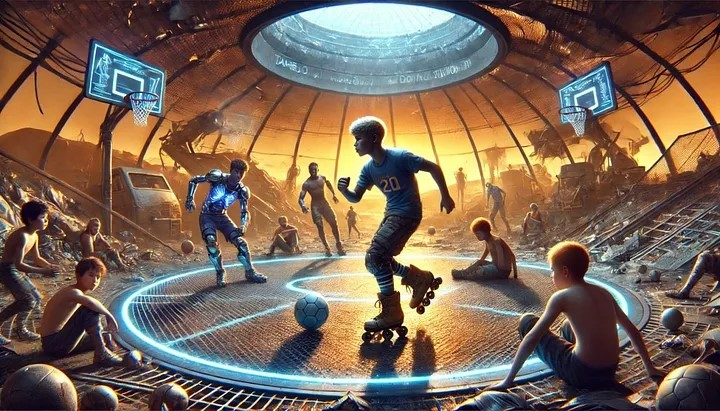
\includegraphics[width=1\linewidth]{img/filho_de_luna.jpg}
\end{figure}

Zé Doidinho acordou sonolento e leu a pichação em neon azul, “também sou filho do dono”. Alguém que dormira ali tinha provavelmente escrito aquilo na parede semidestruída. Aquela frase o motivou.

O lixão de material metálico onde dormia cintilava com um brilho intenso que o cegava. Era um jovem esperto, sobreviver sem morar em um condapt e sem progenitores em Luna é para poucos. Calçou seus patins surrados e correu em alta velocidade para a quadra de entretenimento.

O sol crescia no horizonte e a redoma de Luna convertia a radiação em uma tonalidade alaranjada. A redoma estava rachada devido à última tentativa de girar Nova Europa, mas ninguém se importava. Nos centros de recreação, que eram oferecidos para socialização entre os humanos, oferecia-se uma ração à base de trigo. Como chegou cedo, foi um dos primeiros a jogar contra outros jovens de sua idade.

O jogo lembrava um futebol na terra, com a diferença de que eram Três contra Três em um espaço relativamente pequeno e era jogado com tacos de aço e patins em um terreno plano magnetizado que facilitava a fixação dos patins devido à baixa gravidade.

Seis jovens jogavam, era um corre-corre destrambelhado. Três humanos não modificados e três com modificações robóticas em partes distintas do corpo. Sentados no canto, outros jovens assistiam ao jogo despreocupados e aguardavam a sua vez de entrar em campo. Não havia adultos ao redor, pois eles não apareciam de dia, encontraram algo enterrado em Luna. Era algo que afetava a reprodução humana, por isso os adultos evitavam andar fora dos prédios do Governo Central.

O mais alto dos jogadores empurrou com seu próprio peso Zé Doidinho e o grude magnético de desfez. Zé Doidinho só não partiu a cabeça no chão porque a grade que cobria os cantos amorteceram sua queda. Seu coração acelerou. Sem pensar muito, com punhos levantados e ódio no olhar, partiu para o ataque contra o oponente que parecia duas vezes mais forte.

— Zé Doidinho será estraçalhado, coitado — disse um jovem que estava aguardando a sua vez de entrar em campo.

— Vamos parar com isso! — Falou quem estava segurando a bola.

— Quebra a espinha ele.

Porém, essa disputa já tinha vencedor. O oponente de Zé Doidinho treinava boxe com seu irmão mais velho. Enquanto um girava socos e pontapés ao vento, o outro procurava uma boa entrada para bater no queixo. Para um lado, tropeçou o magricela, cambaleando, para o outro, a pistola laser que Zé Doidinho carregava na cintura. O que era euforia virou espanto.

O trabuco caiu a uma pequena distância. Em poucos segundos, a dúvida dos outros era ficar ou correr. Rapidamente Zé Doidinho o pegou e colocou na cintura. Não lhe passara em nenhum momento usá-lo. Recebera um murro e estava envergonhado, mas sua pistola não era para brincadeiras. Era uma garantia de que teria o que quisesse quando o momento fosse oportuno. Foi um presente de seu tio, Cabeleira. Seu tio pediu para guardar enquanto fugia de uns problemas antigos da terra-dois, que não lhe foram bem explicados.

Com o laser guardado, Zé Doidinho rapidamente se levantou, limpou um pouco do sangue da boca e voltou a trocar murros. Todos os outros estavam paralisados, o que acontecera estava além de seus eventos diários. Devido ao susto, o jogo acabou. Em algum momento, ambos se afastaram e começaram a se xingar.

Alguns meses depois, Zé Doidinho foi perfurado pela polícia de Luna, quando estava em cima de uma estrutura metálica, prestes a saltar por cima de um condapt. Ele roubara um filhote de gato-do-céu, um híbrido de felino e chimpanzé, muito desejado em Nova Europa.

A ideia era vender o animalzinho e fazer uns trocados para uma nova moradia. Foi tudo rápido, ele viu uma oportunidade, pulou o muro e saiu com o filhote debaixo do braço, correndo com seus patins. Porém, logo em seguida, foi perseguido por homens que saíram em sua procura. Por azar, no dia anterior, ele havia emprestado sua pistola para um dos irmãos-vida-louca que disseram que iriam devolver no mesmo dia.

Zé Doidinho não queria ter quebrado a confiança de seu tio, foi seu último pensamento enquanto seu sangue escorria para um bueiro misturado com o musgo da calçada.

Rapidamente a polícia de Luna apareceu e levaram seu corpo para o departamento de pesquisa e inovação.

— Há quanto tempo ele morreu — disse um homem alto coberto com uma roupa extremamente branca da cabeça aos pés.

— A pouco menos de meia hora.

— O cérebro continua relativamente preservado, retirem-no. Descartem o corpo em algum lugar em Nova Europa.

%%%%%%%%%%%%%%%%%%%%
%%%% CAPÍTULO %%%%%%
%%%%%%%%%%%%%%%%%%%%

\chapter{O Sacrifício}

\epigraph{A coragem não é a ausência de medo, mas o triunfo sobre ele}{Aristóteles}

\begin{figure}[h!]
    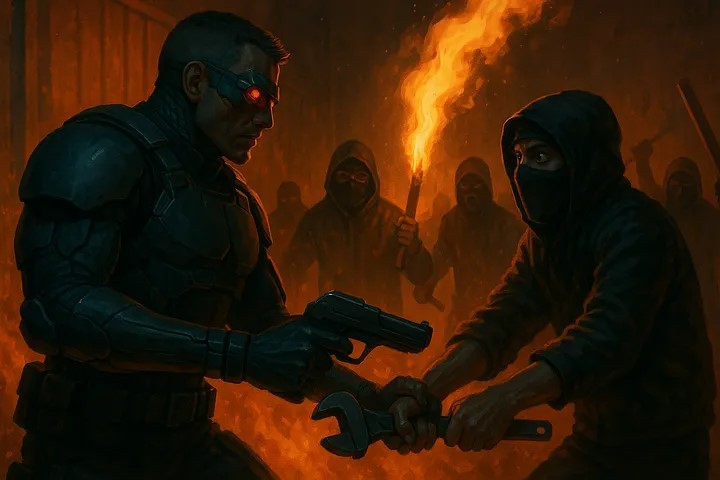
\includegraphics[width=1\linewidth]{img/o_sacrificio.jpg}
\end{figure}

Gustavo iniciava mais uma patrulha de olhos bem abertos. Era um segurança treinado para fornecer força de nível militar para corporações ricas o suficiente para comprá-lo. Enquanto caminhava em sua ronda, ele percebe que o zumbido fraco da maquinaria da cidade é interrompido pelo som de metal retorcido.

Gustavo se vira para ver um grupo de manifestantes, seus rostos mascarados, tentando arrombar o contêiner de transporte do rico empresário. Um deles atira um coquetel molotov em direção ao contêiner.

As chamas iluminam a noite, lançando longas sombras nos rostos dos manifestantes. Eles empunham chaves inglesas, canos e bombas incendiárias. Lutavam por melhores condições de trabalho.

Gustavo correu em direção aos manifestantes, seus passos ecoando na calçada. As chamas do coquetel molotov piscaram nos sensores ópticos conforme ele se aproximava. Uma das figuras mascaradas se vira com uma chave-inglesa na mão. Gustavo estende a mão e agarra o pulso deles, sentindo o metal frio da ferramenta contra sua pele sintética, seu treinamento em artes marciais avançado era obrigatório entre os patrulhadores. Os olhos do manifestante se arregalam de surpresa.

Gustavo interrompe solta o pulso do manifestante. Os olhos dele se estreitam em suspeita enquanto o criminoso recua, colocando uma distância entre ambos. Os outros baderneiros param, observando atentamente. O crepitar das chamas e os sons distantes da cidade enchem o ar. Gustavo sente o calor do fogo em sua pele coberta por escamas sintéticas e percebe que tem uma escolha a fazer. Enquanto Gustavo considera suas opções, saca sua pistola laser, sentindo a suave sensação de poder familiar em sua mão. As expressões dos manifestantes mudam, dava para sentir o medo em seus olhos.

O preparado segurança mira sua pistola no grupo de manifestantes e o ponto vermelho do sistema de mira dança por entre a multidão. Ele aperta o gatilho e um raio brilhante de energia é disparado, cortando o ar com um chiado. O raio atinge um dos manifestantes, que solta um grito de dor enquanto é lançado para trás, caindo no asfalto. Os outros manifestantes ficam congelados no lugar por um instante. Subitamente saem de seu estupor e se dispersam, desaparecendo nas sombras. Deixando Gustavo sozinho com o manifestante ferido.

Gustavo coloca o pé no pescoço manifestante ferido, sua pistola laser ainda apontada para ele. As chamas do coquetel molotov lançam um brilho assustador ao redor da cena. O manifestante geme de dor, segurando com a mão em seu peito esquerdo onde o raio laser atingiu.

Apesar da animosidade que Gustavo sente pelos baderneiros, ele ainda não consegue acabar com a vida deles a sangue-frio. Ele baixa a pistola laser, tomando uma decisão. Os olhos do manifestante ferido estão arregalados de medo, e ele choraminga baixinho. Gustavo decide poupar a vida dele, optando por pedir assistência médica. O corpo do manifestante relaxa visivelmente, o alívio toma conta de suas feições ao perceber que recebeu uma segunda chance.

Gustavo contata rapidamente os serviços de emergência da cidade, solicitando atendimento médico para o manifestante ferido. Enquanto espera a ajuda chegar, ele fica de guarda, garantindo que a cena permaneça segura e protegida. Porém, de súbito, Gustavo ouve passos se aproximando. Seus sensores ópticos examinam a área e ele avista um grupo de figuras se movendo em sua direção com movimento mais deliberados e ameaçadores.

Conforme o grupo avança, Gustavo levanta sua pistola laser, pronto para se defender. Mas antes que ele possa reagir, um deles atira uma granada. Gustavo tenta desviar, mas ela detona ao seu lado, enviando uma onda de choque de força pelo ar. Gustavo sente seu braço se afastar do seu corpo, uma explosão de faíscas e fumaça saindo das peles, ossos e músculos. Sua esposa não lhe receberá em casa hoje para o jantar, pensou, ao menos não inteiro.

Gustavo acordou no hospital ao lado de sua amada esposa.

- Querida, onde está nosso filho? — perguntou Gustavo.

- Ele levou um tiro no peito durante uma rebelião com os amigos, mas está descansando. — respondeu sua esposa demonstrando estar aliviada.

Depois disso, Gustavo dormiu profundamente. Dormiu como nunca tinha feito antes, o sono dos justos. A falta de um braço não era nada mais, próteses biônicas ainda trazem novos recursos.

%%%%%%%%%%%%%%%%%%%%
%%%% CAPÍTULO %%%%%%
%%%%%%%%%%%%%%%%%%%%

\chapter{A Galera do Virote}

\epigraph{“Não preciso de ninguém para fazer merda comigo” (Música MC Pierre)}

\begin{figure}[h!]
    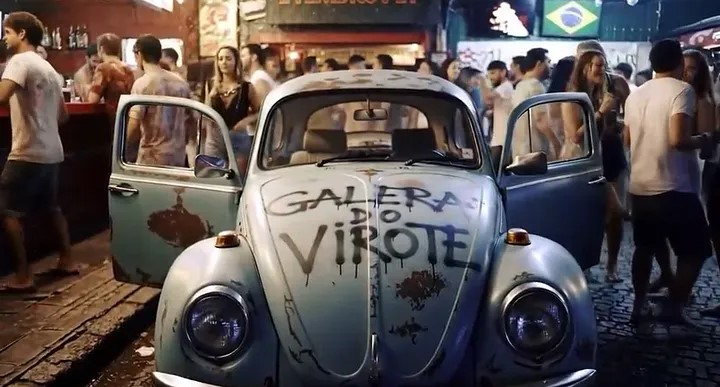
\includegraphics[width=1\linewidth]{img/galera_do_virote.jpg}
\end{figure}

Na cidade de Recife, um grupo de três irmãos, adultos jovens e irresponsáveis, realizava pequenos delitos, roubavam revistas pornôs em banca de jornal e, outras vezes, balas e bebidas de supermercados. Chegaram a invadir uma empresa petrolífera para surfar sandboard nas dunas de Recife. Muitas vezes, saíam sem pagar de pequenos comerciantes. Andavam desafiando a lei e a ordem. Se achavam os maiorais.

A galera do virote era esperta, era sagaz. Com um carro velho e uma moto, seguiam em busca de aventuras. Em um determinado dia, esbanjavam dinheiro para o alto e corriam à noite. Enganaram um policial de trânsito se passando por militares, mijaram na rua — para o horror de senhoras que passavam no momento. O mundo era deles, a noite, um parque de diversões.

Neste dia eram os três jovens e três garotas menores de idade.

— Sei o que elas querem: droga em troca de sexo, vou buscar a cocaína e volto logo. — falou o mais velho da turma.

— A noite é uma criança — falou o mais novo.

— Hoje vamos botar pra quebrar. — e todos riam.

Quando a polícia chegou, levaram todos em cana. Os policiais já iam chegar atirando; ninguém quer arriscar sua vida à toa por vagabundo, pois poderiam estar armados. Mas como estavam em um posto de combustível que tinha câmeras e era bem movimentado, os policiais resolveram entrar com uma abordagem padrão: tapa na cara e algemas.

Os três foram acusados de terem assaltado uma lanchonete, as garotas liberadas. Não era verdade, estavam só bebendo a mais de 24 horas, mas não importava. Depois que foram presos em via pública, zombado de autoridades e incomodando moradores de bairro nobre, terem sidos levados a delegacia era, na verdade, um golpe de sorte.

Ao chegarem na delegacia foram trancafiados em uma pequena cela. Um dos presos mais antigos disse ao mais jovem do grupo para tirar o short e vestir outro que foi jogado pelo mais experiente marginal. Rapidamente, a alegria se transformou em medo e o futuro próspero em consequência.

Este foi a primeira ida e vinda deste grupo naquela delegacia, ficariam conhecidos desde aquele dia pelos policiais como a “Gangue do Virote”.

Um deles morreu cedo, o mais jovem, estava em fuga da polícia depois de um assalto a uma farmácia. Levou um tiro na perna que dilacerou sua veia femoral. Ficou rodando por diversas horas no camburão da polícia antes de ser levado ao hospital, perdeu muito sangue. Não foi dessa vez que a sorte lhe favoreceu.

Outro um pouco mais velho virou bandido de carreira, matou o filho de um advogado da região em troca de um celular, devia dinheiro a traficantes e sua única fonte de receita era o assalto. Era matar ou morrer. Sua morte já era certa, não havia escapatória, se escondeu em um barraco, tremendo e rezando, foi encontrado rapidamente por policiais bem preparados, trocou tiros com a polícia, porém, o desequilíbrio de forças era evidente, velório com caixão fechado.

No velório do irmão mais velho da gangue do virote, havia um certo alívio para os familiares mais distantes que nunca vieram saber como estava a sua vida, nem a dos seus irmãos. No funeral, o comentário era de que ele já foi tarde, pois tinha envergonhado a família. Seu núcleo familiar mais próximo não estava presente, sua mãe falecida há bastante tempo e seu pai alcoólatra, que o criou a socos e tapas, estava desaparecido.

A estupidez da juventude desorientada é maior que sua capacidade de autopreservação. Todos se achavam imortais e os maiorais. Viviam se drogando em busca de felicidade, fugindo de dores inúmeras causadas pela vida cotidiana. Uma mãe morta, um irmão doente, um pai violento, a dor de perder um amigo, a solidão, o estupro, o preconceito.

A centelha do ímpeto da juventude se fazia presente na gangue do virote. Não eram pessoas importantes para ninguém, eram vistos como insignificantes por eles próprios. Ninguém virou médico, professor nem policial. Eram simples marginais, causando problemas para a sociedade.

Um deles, o do meio, sobreviveu à adolescência. Foi morar em outro país, falando outra língua. Longe da influência do meio, seu potencial se realizou. Hoje ele tem um orfanato e cuida de crianças carentes em outro continente. Ele ensina através do esporte como canalizar essa vontade de viver em ações que desenvolvam valores e comportamentos mais produtivos para a sociedade. Sua instituição de caridade hoje é chamada de “Galera do Esporte”.

%%%%%%%%%%%%%%%%%%%%
%%%% CAPÍTULO %%%%%%
%%%%%%%%%%%%%%%%%%%%

\chapter{Esqueci meu carro}

\epigraph{Hoje, \\
que as memórias se esvaem \\
e os amigos fogem de mim, \\
só tenho minhas poesias \\
como amigas \\
confidentes, \\
mesmo assim, \\
impertinentes, \\ 
sem rima e vazias \\
não inspiram a menor confiança: \\
elas também me traem.}{Ivone Boechat}

\begin{figure}[h!]
    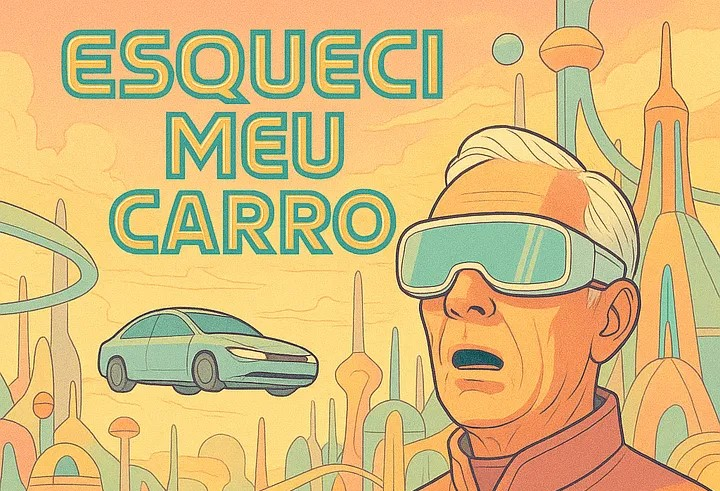
\includegraphics[width=1\linewidth]{img/esqueci_meu_carro.jpg}
\end{figure}

Eu estava em casa conversando com conhecidos e abri o vidi-fone no aplicativo de notícias individuais do momento. Na tela, projetada na retina, como em um jogo de cassino, ao rolar os olhos para baixo apareceu uma nova notificação. Era o vídeo de um amigo curtindo a vida? Não, mas era um vídeo de um idoso sorridente por volta dos 70 anos.

— Existe idade para tudo. Amanhã, vou tirar minha carteira de motorista — dizia com empolgação o futuro habilitado na imagem projetada em minha retina, e continuou: — Achei este carro no estacionamento do shopping e, como ninguém apareceu para reclamá-lo, decidi que vou aprender a dirigir e ficar com ele. Já não era sem tempo. Sempre sonhei em dirigir.

Ao analisar melhor o vídeo, depois de alguns zooms, percebi que era o meu carro, o qual tinha perdido há alguns meses. Não me recordava quando nem onde. Depois de viajar por muitas cidades, a memória já não era mais a mesma. Porém, realmente era o veículo de estimação. Tenho dois, e um deles eu havia esquecido em algum lugar. Falei com o secretário ao telefone que prontamente confirmou, eu tinha perdido aquele carro fazia poucos meses.

No vidi-fone, iniciei uma chamada de voz para o sorridente.

— Cidadão, este carro é meu, não tire sua carteira de motorista, irei buscá-lo assim que possível. — falei com entusiasmo.

— Eu encontrei o carro há uma semana, ele está na oficina consertando. — retrucou o idoso.

— O carro é novo e está em ótimas condições. Portanto, não precisa de conserto.

— Mas ele não ligava, quando eu o encontrei.

— Provavelmente porque a bateria descarregou. Irei amanhã mesmo pegá-lo.

O idoso ficou apático, sua felicidade tinha desaparecido. Infelizmente para ele, o sonho acabou. Mas para mim restava o regozijo. Resgatei meu bem precioso. Nos dias de hoje, um bem como este custa quase o preço de um rim. É justo que os bens retornem para o uso de seus proprietários.

O idoso ainda falou algo sobre “achado não é roubado”. Mas não havia lei que desse respaldo a seus argumentos. Fingi-me de cidadão conhecedor de direitos e disse que iria pegar o veículo amanhã mesmo e que, caso ele se recusasse, eu levaria a polícia.

Falei com o secretário, que prontamente irá viajar para resgatar o veículo. Nos meus 90 anos de idade, ainda espero com saudade colocar as mãos no seminovo que comprei, mas não me lembro onde… nem quando…


\end{document}